\documentclass[10pt]{article}
\usepackage{icmlko}

\icmlmeta{IP 파운데이션 월드모델}{309}{빌리던 도메인에 제 축을 준다}{펀딩에 전용 범주 축을 만들어 넣었다 --- 도메인은 크게 올랐는데 빌림은 안 물러났다}

\begin{document}

\twocolumn[
\icmlheader

\begin{abstract}
노트 303이 ``도서 · 펀딩에 축을 더 --- 빌릴 자리가 있다는 뜻''을 남겼다.
오늘은 \textbf{재는 쪽이 아니라 짓는 쪽}을 골랐다. 뒤졌더니
\texttt{funding\_axes.json} 의 \texttt{category} 가 축으로 안 쓰이고 있었고
(덮음 100\% · 값 스무 가지), \textbf{채택 검사 셋을 다 통과한다} ---
① 크루스칼 $H{=}56.7$($p{<}$1e-4, 연도 통제 후 30.5) · ② 시간 조각 다섯
부호 일치 \textbf{5/5} · ③ 공유 축을 통제한 잔차에서 $H{=}42.2$($p{=}0.0001$).
무리 순서가 \texttt{publication > webtoon-resources > food > $\ldots$ >
apparels} 로, 이 실험실이 재려는 방향(IP 를 업은 정도)과 같다.
\texttt{lab/fundaxes.py} 로 만들어 넣고 쟀다. \textbf{펀딩 0.2536 $\to$
0.3709}($+$0.1173 · 짝SE 0.0518 · $t{=}{+}2.27$) --- \textbf{제 검출 문턱
0.1036 을 넘는다.} 판은 0.4799 $\to$ 0.4822($+$0.0023 · $t{=}1.24$)로
\textbf{못 가른다}(펀딩이 판의 3\%다 --- 미리 그렇게 적었다). 가드 전부 통과.
\textbf{그런데 진짜 시험은 딴 데 있었다.} 노트 303의 ``대타'' 읽기가 맞다면
제 축이 생길 때 \textbf{빌림이 물러나야} 한다. 갈라 보니 \textbf{안
물러났다} --- 빌린 \emph{양}은 0.1089 $\to$ 0.0965($-$11\%, 짝SE 0.05 라 0 과
못 가름)이고 줄어든 것은 \emph{몫}(43\% $\to$ 26\%)뿐이다. \textbf{분모가
커진 것이지 빌림이 물러난 것이 아니다.} 제 것과 빌린 것은 \textbf{대체가
아니라 덧셈}이다.
\end{abstract}
]

\section{짓는 쪽을 골랐다}

노트 303의 ``남은 것'' 첫 줄이 ``도서 · 펀딩에 축을 더''였다. 오늘까지
열여섯 노트가 전부 \emph{재는} 일이었다. 뒤졌다.

\begin{center}\footnotesize
\begin{tabular}{lll}
\hline
도메인 & 안 쓰인 재료 & 판정 \\
\hline
도서 & \texttt{publisher} & 5건 이상 무리가 셋 · ① 탈락 \\
\textbf{펀딩} & \texttt{category} & \textbf{①②③ 전부 통과} \\
펀딩 & \texttt{creator} & 287가지 · 무리 부족 \\
\hline
\end{tabular}
\end{center}

\paragraph{채택 검사 셋} 전부 학습 구간이고 유보를 안 봤다(노트 239 · 285).

\begin{center}\footnotesize
\begin{tabular}{ll}
\hline
① 혼자 가르나 & $H{=}56.7$ ($p{<}$1e-4) \\
\quad 연도 통제 후 & $H{=}30.5$ ($p{<}$1e-4) \\
② 시간 조각 다섯 & \textbf{부호 일치 5/5} (조각마다 $n{=}64$) \\
\quad 순위 상관 & .200 · .900 · .600 · .800 · .200 \\
③ 기존 축과 겹침 & 잔차에서 $H{=}42.2$ ($p{=}0.0001$) \\
\hline
\end{tabular}
\end{center}

무리 순서가 \textbf{publication > webtoon-resources > food > home-and-living
> perfumes-and-beauty > apparels} 다. 위가 IP · 출판 쪽이고 아래가 상품 쪽
--- 이 실험실이 재려는 축과 같은 방향이다.

\paragraph{설계} 전용 이름(노트 250 · 251) · 눈금은 집단 크기만 쓰므로
라벨을 안 본다 · 15건 미만 무리는 마스크 0(열두 무리 · 마스크 93\%) ·
펀딩 학습 320행이라 F18 청력 22를 넘는다 · \texttt{provenance} 에 PRE 로
등록(\texttt{mkt\_cat} 도 등록이 빠져 있어 같이 넣었다).

\section{펀딩이 문턱을 넘는다}

\begin{figure*}[t]
\centering
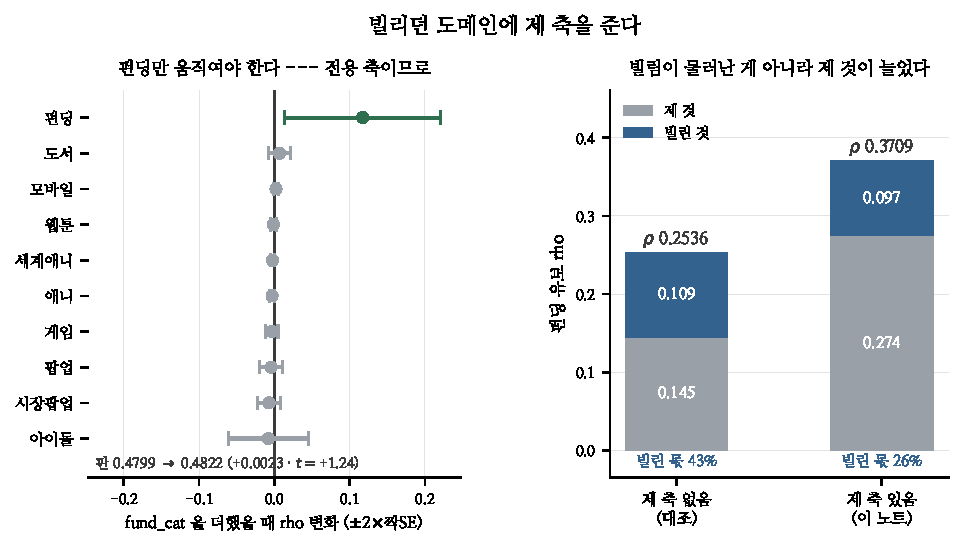
\includegraphics[width=\textwidth]{figs/own.pdf}
\caption{왼쪽 --- \texttt{fund\_cat} 을 더했을 때 도메인 $\rho$ 의 변화
($\pm$2$\times$짝SE). 오른쪽 --- 펀딩의 유보 $\rho$ 를 제 것과 빌린 것으로
가른 것.}
\end{figure*}

\begin{center}\small
\begin{tabular}{lrrr}
\hline
& 기준 & 새 & $t$ \\
\hline
\textbf{펀딩} & 0.2536 & \textbf{0.3709} & \textbf{$+$2.27} \\
도서 & 0.3895 & 0.3964 & $+$0.92 \\
모바일 & 0.5464 & 0.5485 & $+$1.33 \\
세계애니 & 0.5475 & 0.5450 & $-$1.85 \\
애니 & 0.4764 & 0.4733 & $-$1.71 \\
나머지 다섯 & \multicolumn{3}{c}{$|t|{<}1.0$} \\
\hline
\textbf{판} & 0.4799 & 0.4822 & $+$1.24 \\
\hline
\end{tabular}
\end{center}

\textbf{펀딩 $+$0.1173 에 짝SE 0.0518} --- 제 검출 문턱 0.1036 을 넘는다.
다만 판 전체를 훑는 다중비교 문턱($|t|{>}2.77$)에는 못 미친다. 미리 적은
예측이 ``$+$0.03 $\sim$ $+$0.10''이었는데 \textbf{그보다 컸다.}

판은 $+$0.0023 으로 못 가른다 --- \textbf{미리 그렇게 적었다.} 펀딩 유보가
80/2,669 즉 3\%라 $0.1173 \times 0.03 = 0.0035$ 가 기대치이고 관측이 그
언저리다. \textbf{판이 도메인 이득을 구조적으로 못 본다}(노트 279 · 300).

배포 규칙(노트 275 · 282)으로는 ① 판이 미결정 띠 안 ② 어느 도메인도
$|t|{>}2.77$ 로 나빠지지 않음 --- \textbf{둘 다 통과}이고 채택 근거는 학습
구간에서 미리 섰다. 가드 열아홉 통과 · 표시자 ``볼 것 없음''.

\section{그런데 빌림이 안 물러났다}

노트 303의 읽기는 ``전이는 대타다 --- 제 신호가 있으면 안 빌리고 없으면
빌린다''였다. 그렇다면 \textbf{제 축이 생기면 빌림이 물러나야} 한다.
그것이 이 노트의 진짜 시험이고 미리 그렇게 적었다.

\begin{center}\small
\begin{tabular}{lrr}
\hline
& 제 축 없음 & 제 축 있음 \\
\hline
펀딩 $\rho$ & 0.2536 & \textbf{0.3709} \\
\quad 제 것 & 0.1447 & \textbf{0.2744} \\
\quad \textbf{빌린 것} & \textbf{0.1089} & \textbf{0.0965} \\
빌린 몫 & 43\% & \textbf{26\%} \\
\hline
\end{tabular}
\end{center}

\textbf{빌린 양은 안 줄었다.} $-$0.0124 는 짝SE 0.05 수준에서 0 과 못
가른다. 줄어든 것은 \textbf{몫}이고, 그건 \emph{분모가 커져서}다.

\begin{center}\small
\begin{tabular}{ll}
\hline
대타라면 & 빌림 $\to$ 0 · 관측 \textbf{0.0965} \\
덧셈이라면 & 빌림 그대로 · 관측 \textbf{$-$0.0124} \\
\hline
\end{tabular}
\end{center}

\textbf{덧셈 쪽이다.} 제 축이 나른 정보와 빌려 온 구조가 \textbf{겹치지
않는다} --- \texttt{fund\_cat} 은 범주이고 빌리는 것은 검색 셋 · 달력 여섯이니
당연하다면 당연하다. 그런데 노트 303의 낱말(``대타'')은 그 둘이 같은 자리를
놓고 다툰다는 뜻이었다. \textbf{그 낱말이 과했다.}

\paragraph{그래서 노트 303을 정정한다}

\begin{center}\footnotesize
\begin{tabular}{ll}
\hline
노트 303 & \textbf{고침} \\
\hline
전이는 대타다 & 전이는 \textbf{보완}이다 \\
제 신호 없으면 빌린다 & 그대로 (관측은 여전히 맞다) \\
제 축이 생기면 물러난다 & \textbf{안 물러난다} \\
\hline
\end{tabular}
\end{center}

\textbf{``제 신호가 없는 도메인만 빌린다''는 관측은 살아 있다} --- 다만
그것이 \emph{제 신호가 빌림을 밀어낸다}는 뜻은 아니었다. 큰 도메인이 안
빌리는 것은 \textbf{빌릴 것이 없어서}일 수도 있다(제 축이 이미 그 자리를
설명해서가 아니라).

\paragraph{남은 것}
\begin{center}\small
\begin{tabular}{ll}
\hline
갈래 & 왜 \\
\hline
큰 도메인에 축을 빼 보면 & 빌림이 생기나 --- 대칭 시험 \\
도서에 줄 축 & \texttt{publisher} 는 떨어졌다 \\
펀딩 유보 80행 & 문턱 0.10 이 너무 높다 \\
\texttt{fund\_cat} 승격 & 배포 규칙 통과 · 판은 못 가름 \\
\hline
\end{tabular}
\end{center}

\paragraph{규약} \textbf{짓고 나서 재면 낱말이 틀린 것을 안다.} 노트 303이
쓴 ``대타''는 관측(빌리는 것은 제 신호 없는 둘뿐)에서 나온 \emph{해석}이었고,
그 해석이 예측을 낳았고(제 축이 생기면 물러난다), \textbf{그 예측이 틀렸다.}
관측은 살고 낱말은 죽는다. 그리고 \textbf{도메인 이득은 판에 안 보인다}
--- 펀딩이 제 문턱을 넘는 $+$0.1173 을 냈는데 판은 $+$0.0023 이다.
\textbf{판만 보고 있었으면 이 축을 안 넣었을 것이다.}

\end{document}
